\documentclass[a4paper]{article}

\usepackage[italian]{babel}
\usepackage[utf8]{inputenc}
\usepackage[T1]{fontenc}
\usepackage{microtype}
\usepackage{xcolor}
\usepackage{titlesec}
\usepackage{xargs}
\usepackage{multicol}

\usepackage{graphicx}

\usepackage{booktabs}

\usepackage[colorlinks]{hyperref}
\definecolor{RoyalBlue}{rgb}{0.0, 0.14, 0.4}
\hypersetup{
     colorlinks=true,
     linkcolor=blue,
     filecolor=blue,
     citecolor = black,
     urlcolor=cyan,}

\title{Algoritmo di bisezione \\ Algoritmo di Newton}
\date{2 maggio 2021}
\author{Davide Peccioli}

\begin{document}
\maketitle

Entrambi questi algoritmi sono utilizzati per calcolare con una buona approssimazione gli zeri di una funzione, quando questi non sono "banali", ovvero calcolabili con puri passaggi algebrici.

In particolar modo, il programma qui presentato prende in input una funzione qualsiasi e, dopo averne stampato il grafico e richiesto all'utente in quale intervallo vi sia \textbf{un solo} zero, calcola questo zero con due algoritmi, in due tempi separati.

Il codice commentato è presente su \href{https://github.com/DavideP02/Scuola_Liceo_5_Informatica_Octave-AnalisiNumerica-Peccioli5H/blob/main/analisi.m}{GitHub}\footnote{https://github.com/DavideP02/Scuola\_Liceo\_5\_Informatica\_Octave-AnalisiNumerica-Peccioli5H/blob/main/analisi.m}.

\section{Algoritmo di bisezione}

L'algoritmo di bisezione, il primo eseguito dal programma, funziona nel seguente modo:
\begin{itemize}
    \item l'utente sceglie un intervallo, tale per cui:
    \begin{itemize}
        \item la funzione è continua e derivabile;
        \item è presente un solo zero;
        \item la funzione, agli estremi dell'intervallo, ha segno discorde;
    \end{itemize}
    \item viene calcolato il punto medio dell'intervallo scelto;
    \item si stabilisce quale dei due intervalli venutisi a formare (\textit{estremo sinistro-punto medio} o \textit{punto medio-estremo destro}) rispetta i requisiti presentati nel punto precedente;
    \item l'algoritmo si ripete con questo "nuovo" intervallo.
\end{itemize}

Così facendo si isolerà con una precisione sempre maggiore l'intervallo in cui è presente lo zero. Non si giungerà \textit{quasi} mai ad un risultato preciso, tale per cui la funzione calcolata nel punto sia esattamente $0$, e pertanto è necessario porre una sensibilità al programma: nel programma qui presentato la sensibilità è impostata a $1\cdot 10^{-15}$.

\section{Algoritmo di Newton}

L'algoritmo di Newton (o delle tangenti), il secondo eseguito dal programma, funziona in modo analogo all'algorimo di bisezione:
\begin{itemize}
\item l'utente sceglie un intervallo, che deve presentare le stesse caratteristiche dell'intervallo scelto per l'algoritmo di bisezione, ma in cui la derivata seconda della funzione deve essere continua e mantenere costante il suo segno;
\item preso il punto estremo con ordinata di segno concorde con quello della derivata seconda, si traccia la retta tangente alla curva in quel punto;
\item la proiezione dell'intersezione della retta con l'asse delle $x$ sulla curva studiata rappresenterà il nuovo estremo dell'intervallo, che sostituirà quello preso in considerazione in precedenza;
\item si itera l'algoritmo fino a che l'intersezione della retta tangente con l'asse delle $x$ presenta un'immagine sufficientemente vicina allo zero (con precisione arbitrariamente scelta).
\end{itemize}

In questo modo, aggiungendo un'ipotesi sull'intervallo scelto, rispetto all'algoritmo di bisezione, è possibile diminuire fortemente il numero di iterazioni.

\section{Funzioni studiate}

Segue una tabella con indicati le funzioni studiate, gli intervalli considerati e il numero di iterazioni necessarie a ciascun algoritmo per trovare la soluzione, data una precisione di $1\cdot 10^{-15}$.
\[
\begin{array}{cccc}
\toprule
\textbf{Funzione} & \textbf{Intervallo} & \textbf{Bisezione} & \textbf{Newton} \\
\midrule
\arctan(x)-x^3 & [-1,2; -0,6] & 47 & 6 \\
\sin(x)-\sqrt{x}+1 & [1,5; 4] & 48 & 10 \\
\log(x)-x^2+1 & [0,2; 0,6] & 46 & 6 \\
x^4+x^3-1 & [-1,8; -1] & 46 & 6 \\
(10-x)\cdot e^{-10x}-x^{10}-1 & [0; 0,4] & 49 & 7 \\
\bottomrule
\end{array}
\]

Come si può notare dalla tabella riportata, l'algoritmo di bisezione impiega un numero di iterazioni ben maggiore rispetto all'algoritmo di Newton, di circa il $600\%$. 

Considerando che la precisione per gli entrambi gli algoritmi è la stessa, e che per comodità per entrambi gli algoritmi viene utilizzato lo stesso intervallo, a prima vista sembrerebbe che l'algoritmo di Newton sia il più efficiente senza ombra di dubbio. Sebbene sia effettivamente l'algoritmo più efficiente, è necessario considerare che utilizzando lo strumento matematico della derivazione, l'algoritmo di Newton impiega più risorse rispetto a quello di bisezione per ogni iterazione fatta.

\begin{figure}
\centering
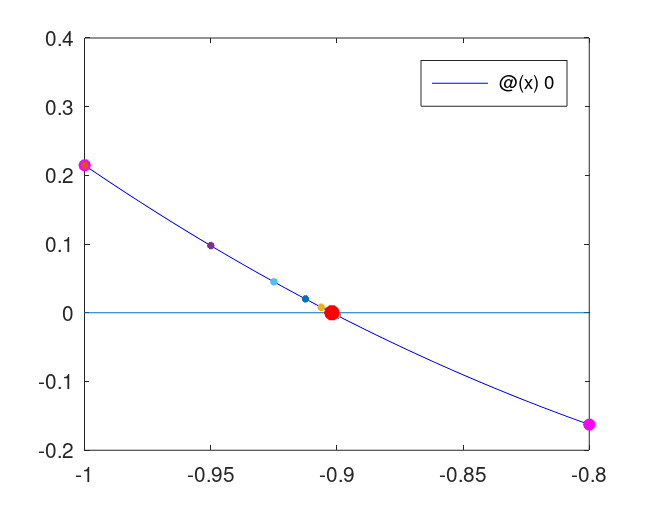
\includegraphics[width=12cm]{Bisezione}
\caption{Punti considerati dall'algoritmo di bisezione per studiare la funzione $\arctan(x)-x^3$}
\label{fig:bis}
\end{figure}
\begin{figure}
\centering
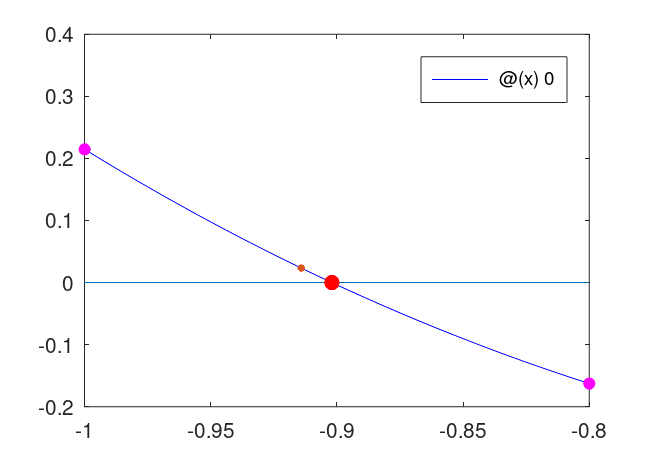
\includegraphics[width=12cm]{Newton}
\caption{Punti considerati dall'algoritmo di Newton per studiare la funzione $\arctan(x)-x^3$}
\label{fig:new}
\end{figure}

\end{document}